\chapter{Limits of Distributions}

\section{Introduction}

In this lab, we will use a Monte Carlo simulation to demonstrate the
convergence of statistical distributions.  We'll see that the binomial
distribution approaches the Poisson distribution for a large number of
trials, and that the Poisson distribution approaches the Gaussian
distribution for a large values of the mean value $\lambda$.  You will
produce your own numerical demonstration of the Central Limit Theorem,
by considering the average value of uniform random variables.

\section{Poisson Limit of the Binomial Distribtion}

We showed in lecture that the Binomial distribution for $n$
independent trials with success probability $\epsilon$ approaches a
Poisson distribution with mean value $\lambda = \epsilon \cdot n$ as $n\to
\infty$.  We will demonstrate this numerically by using a large but
finite value for the number of trials $n$.

A simulation of a binomial process is demonstrated in
Fig.~\ref{fig:binom} which will be a good start for the exercises.
While working through the example, note a few key features:
\begin{itemize}

\item Note the distinction between the number of trials {\tt NTRY} and
  the number of random throws {\tt THROWS}.  The simulation throws
  {\tt THROWS} random variables $m$ each of which represents the
  outcome of an binomial process with {\tt NTRY} trials.  It's easy to
  get these quantities confused!

\item The simulated binomial outcomes are contained in the array {\tt
  m} which is filled by calling the \\ {\tt np.random.binomial}
  function which is designed for this specific purpose.  It produces
  an array of the specified size containing values randomly drawn from the
  binomial distribution with {\tt n} trials of {\tt p} success probability.
  Here the computing languages uses {\tt p} for the parameter we call
  $\epsilon$.  That's life!

\item We want to keep the parameter $\lambda$ constant as we vary $n$ so we set the success probability $\epsilon = \lambda / n$ with the line {\tt EPS = LAMBDA / NTRY}.

\item We calculate and plot a histogram in much the same way as in
  previous exercises.  But notice that instead of center of each bin,
  we bplot using the left edge of each bin, determined as {\tt lbins =
    bins[:-1]}.  The reason for this choice is described in more
  detail below.

\item We compare our simulated outcomes to the probability mass function (PMF) for the Binomial process evaluated at the integer values in the array {\tt lbins}

\item The prediction for each bin is normalized by multiplying the PMF (which represents a single throw) by the number of throws {\tt THROWS}.  There is no factor for the bin size in this normalization, because the bin size is 1.

  
\end{itemize}

{\bf Binning integer data:} when plotting a histogram filled from
continuous data, we plotted the count for each bin over the central
$x$ value for the bin.  So the number of entries in the range $[0,1)$
would be plotted over the value $0.5$.  This is a good choice for
continuous data, because continuous data fills the entire range
$[0,1)$.  But in this example, our random variables are integers.  The
only value that can increment the bin at $[0,1)$ is the value
(the range is open on the right, and does not include 1, which is left
for the next bin!)  In this case, it is misleading to plot a count
of the value 0 over the center of the bin at 0.5.  Instead, when
plotting histograms of integer data with integer bins, we plot the
data over the left edge of the bin.  For example, the count of 0
values will be placed directly over 0.

\begin{samepage}
\begin{plot} \end{plot}
Adjust the example code so that the simulated binomial process is
compared to the Poisson PMF instead of the binomial PMF.  Look up the
{\tt np.stats.poisson.pmf} function.  {\bf Make sure that you leave
  the simulation unchanged:} the point of this exercise is to simulate
a binomial process but compare it to a Poisson PDF.  Leave the number
of trials (and other parameters) unchanged.  The agreement between the
Binomial simulation and the Poisson PDF should not agree for six
trials.  Do your results here confirm that?
\end{samepage}

\begin{samepage}
\begin{plot} \end{plot}
Increase the number of trials in your simulated process to 100.  Does
your binomial process now resemble a Poisson PDF?
\end{samepage}

\begin{figure}[htbp]
\begin{center}
  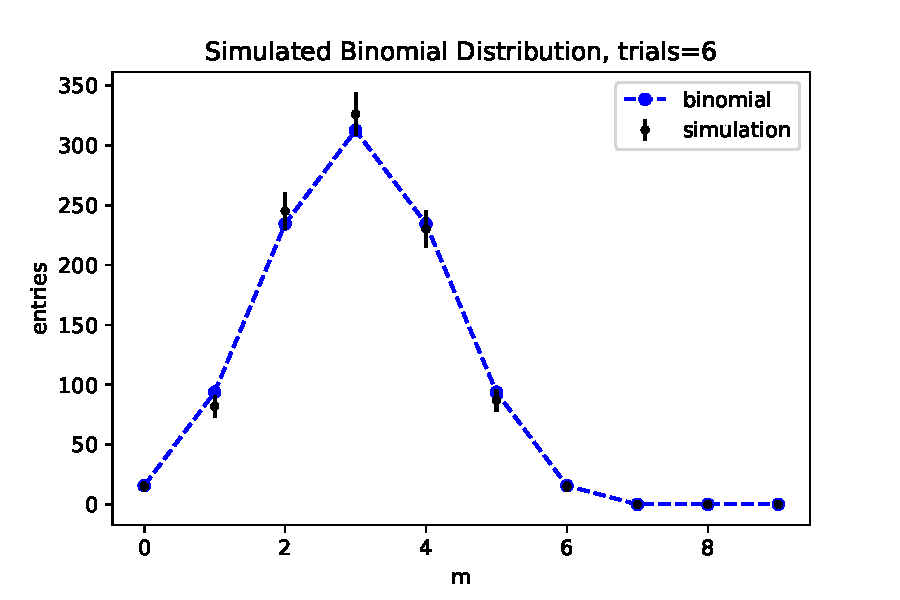
\includegraphics[width=0.50\textwidth]{figs/limits/binomial.pdf}
  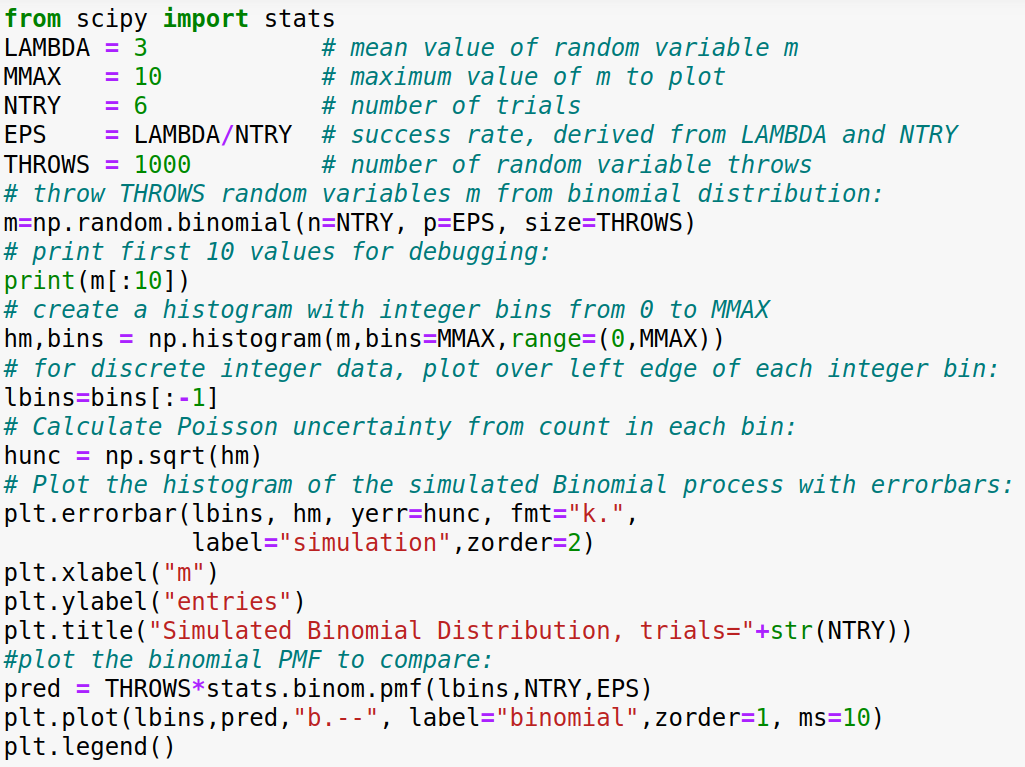
\includegraphics[width=0.75\textwidth]{figs/limits/binomial-code.png} 
\caption{Simulation of a binomial process.}
\label{fig:binom}
\end{center}
\end{figure}

\section{Gaussian Limit of the Poisson Distribtion}

We discussed in lecture that in the limit $\lambda \to \infty$, the
Poisson distribution will approach a Gaussian distribution with mean
value $\lambda$ and $\sigma = \sqrt{\lambda}$.  We will demonstrate
this result numerically using a simulated Poisson process and a large
but finite value of $\lambda$.

A simulation of a Poisson process is demonstrated in
Fig.~\ref{fig:poisson}, which is similar in many respects to the
previous example.  Note a few features:
\begin{itemize}
\item The simulated Poisson outcomes are contained in the array {\tt
  m} which is filled by calling the \\ {\tt np.random.poisson}
  function which is designed for this specific purpose.  It produces
  an array of the specified size containing values drawn from the
  poisson distribution with mean {\tt lam} (the parameter we call
  $\lambda$).

\item The $x$-values used as locations to plot the histogram counts
  are contained in the array {\tt ibins}.  These are determined from
  the bin edges as the largest integer smaller than the center of the
  bin.  This reduces to the left edge for integer bins (as in the
  previous example) but will continue to work as the bin size
  increases to include multiple integers.

\item The outcomes are now being compared to the continuous Gaussian
  PDF.  For this reason, a finely binned set of of $x$-values are
  contained in the {\tt xf} array, filled using the {\tt np.linspace}
  function.  This will plot a nice smooth function, appropriate for a
  continuous function.
  
\item The prediction is normalized by multiplying the PDF (which
  represents a single throw) by the number of throws {\tt THROWS} and
  the bin size.  The bin size factor is needed because we are using a
  probability density function and the bin size will be different than
  one in the exercises.

\item The parameters for the Gaussian PDF are poorly choosen in the
  example, on purpose.
\end{itemize}

\begin{plot} \end{plot}
Lookup the function {\tt scipy.status.norm.pdf}.  Set the parameters
{\tt loc} and {\tt scale} to values consistent with the simulation.
Leave $\lambda=3$ for now and plot your results.  How does the Gaussian distribution compare to Poisson distribution at $\lambda=3$?

\begin{plot} \end{plot}
Now set $\lambda=100$.  Adjust the range for plotting to $[70,130]$ and set the number of bins to 20.
The Gaussian distribution distribution should agree closely with the Poisson distribution at this point.  Is that what your simulation shows?

\begin{figure}[htbp]
\begin{center}
  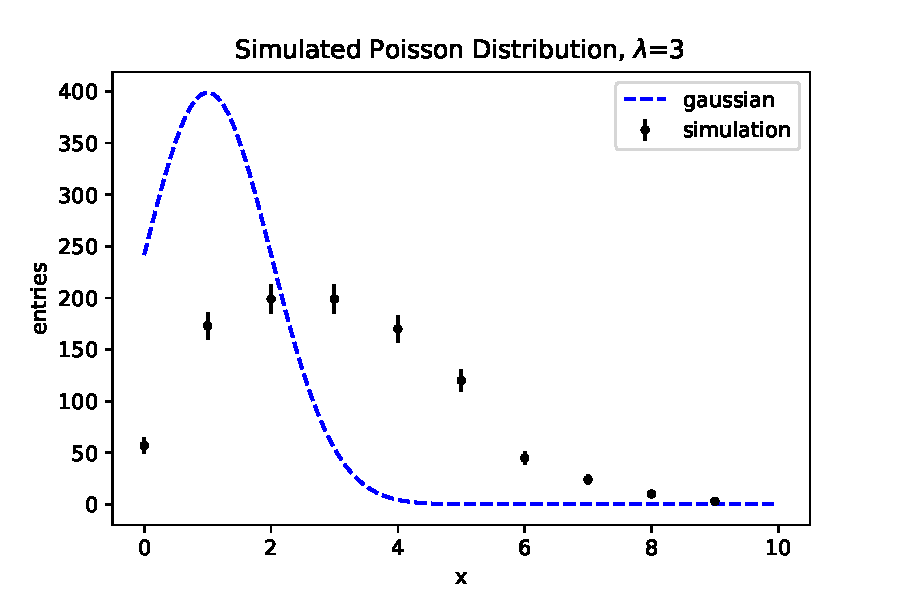
\includegraphics[width=0.50\textwidth]{figs/limits/poisson.pdf}
  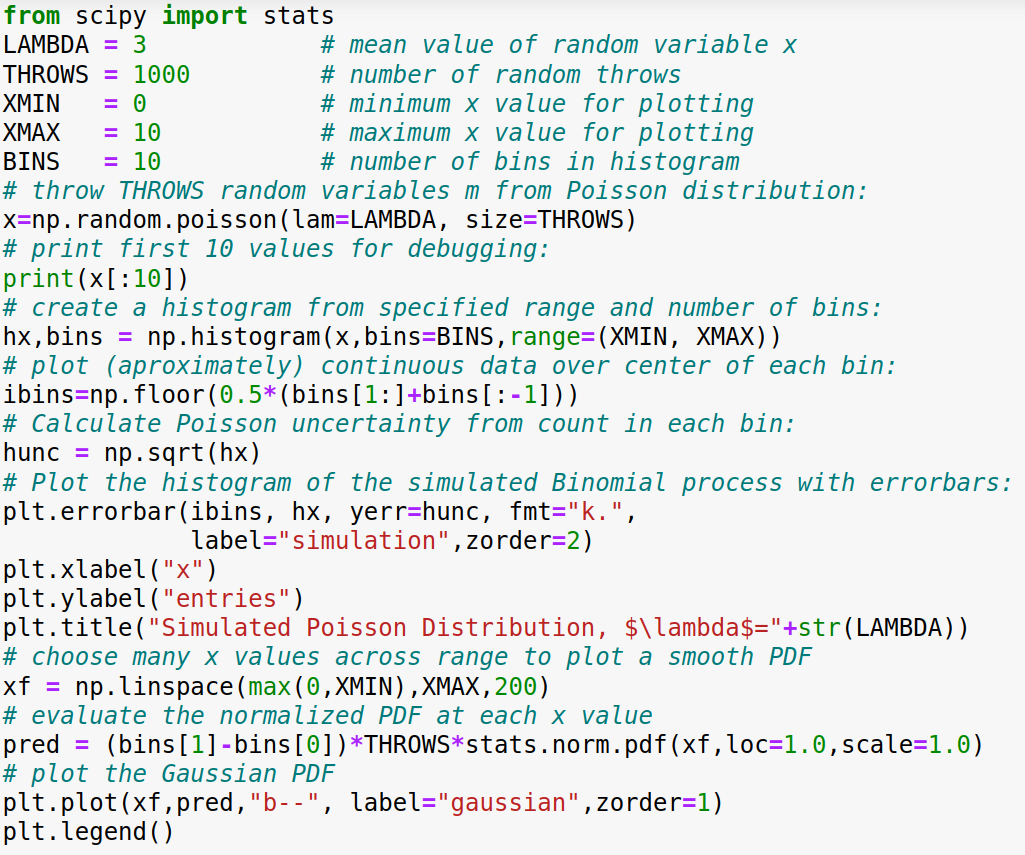
\includegraphics[width=0.75\textwidth]{figs/limits/poisson-code.png} 
\caption{Simulation of a binomial process.}
\label{fig:poisson}
\end{center}
\end{figure}


\section{The Central Limit Theorem}

The central limit theorem states that a properly normalized sum of
independent random variables will tend toward the Gaussian
distribution, even if the random variables are drawn from a different
distribution.  In this section, you will demonstrate this fact by
showing that the average of {\tt NSUM} uniform random variables does
in fact follow a Gaussian distribution.

When solving these exercises, you should consider the following points:
\begin{itemize}

\item You'll want to simulate a large number {\tt THROWS} of average
  values, where each avearge value is based on {\tt NSUM} individual
  uniform random variables.  Produce your uniform random variables in
  the range $[-1,1]$ using the {\tt np.random.uniform} function.

\item As all of the variables in this section are continuous, you should use
the bin centers when plotting histograms, as in previous labs, calculated as
{\tt cbins = (bins[1:] + bins[:-1])/2}.

\item You will be comparing your simulated results to the Gaussian
  PDF.  The best estimates for the mean and variance of the Gaussian
  from our sample of simulated data is provided by the sample mean and
  sample variance, which are calculated by the {\tt np.mean} and {\tt
    np.var} funtions.  Make sure to normalize your PDF to obtain your
  prediction.

\end{itemize}

\begin{plot} \end{plot}
Generate {\tt THROWS=10000} averages of {\tt NSUM=100} random
variables thrown from uniform distribution in the range $[-1,1]$.
Plot a histogram of these average values across an appropriate range
that clearly shows the bell shaped Gaussian distribution, using about
50 bins.  On the same axes, plot a Gaussian PDF, appropriately
normalized, to compare with your simulation.

\begin{plot} \end{plot}
Using the statistical concepts we developed in lecture, you should be
able to calculate, with pencil, the expected mean and variance of the
average values.  Determine these predicted values and compare
the values reported by {\tt np.var} and {\tt np.mean} for your
simulation.
